\section{Synthesis}
Finally, the VHDL design has been synthetized for the ZyBo board. This section
reports the main metrics: timing, power and utilization.

\subsection{Timing}
\begin{center}\vspace*{\baselineskip}
    \def\arraystretch{1.5}
    \begin{tabular}{|c|c|}\hline
        \textbf{Setup Worst Negative Slack (WNS)} & 57.119\si{\nano\second}\\\hline
        \textbf{Setup Total Negative Slack (TNS)} & 0.000\si{\nano\second}\\\hline
        \textbf{Worst Hold Slack (WHS)} & 0.215\si{\nano\second}\\\hline
        \textbf{Total Hold Slack (THS)} & 0.000\si{\nano\second}\\\hline
    \end{tabular}\vspace*{\baselineskip}
\end{center}

Since the clock frequency was set at 16\si{\mega\hertz}, the bottleneck path 
is $62.5-57.119 = 5.381 \si{\nano\second}$ long and therefore the maximum operating
frequency is $1/5.381 \simeq 185 \si{\mega\hertz}$. However, there is no point 
in going too fast since it would just increase the power consumption (samples come 
in at a 16\si{\kilo\hertz} rate).

The bottleneck path is represented by the multiplier that is used to square the 
sample, hence using the approximated absolute value brings no benefit to timing.

\subsection{Power}
The power report has been generated in Vivado using the default settings.

\begin{center}\vspace*{\baselineskip}
    \def\arraystretch{1.5}
    \begin{tabular}{|c|c|}\hline
        \textbf{Total On-Chip Power} & 0.09\si{\watt}\\\hline
        \textbf{Junction Temperature} & 26.0\si{\celsius}\\\hline
        \textbf{Thermal Margin} & 59.0\si{\celsius} (5.0\si{\watt})\\\hline
        \textbf{Effective $\theta$\si{\joule\ampere}} & 11.5\si{\celsius/\watt}\\\hline
        \textbf{Power supplied to off-chip devices} & 0\si{\watt}\\\hline
        \textbf{Confidence level} & Low\\\hline
    \end{tabular}\vspace*{\baselineskip}
\end{center}

\begin{figure}[h!]
    \centering
    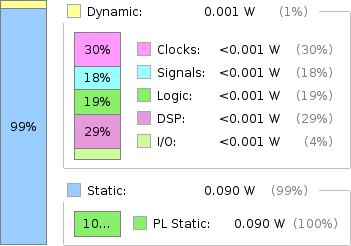
\includegraphics[width=0.5\textwidth]{figs/power_report_master.png}
    \caption{Power report}
    \label{fig:power_master}
\end{figure}

\subsection{Utilization}
\begin{center}\vspace*{\baselineskip}
    \def\arraystretch{1.5}
    \begin{tabular}{|c|c|c|c|c|}\hline
        \textbf{Resource} & \textbf{Utilization} & 
        \textbf{Utilization ``opt''} & \textbf{Difference} & 
        \textbf{Available}\\\hline
        LUT & 118  (0.67\%) & 110   (0.63\%) & \textbf{8} & 17600 \\\hline
        FF  &  74  (0.21\%) &  73   (0.21\%) & \textbf{1} & 35200 \\\hline
        DSP &   1  (1.25\%) &   1   (1.25\%) & 0          &    80 \\\hline
        IO  &  20 (20.00\%) &  20  (20.00\%) & 0          &   100 \\\hline
    \end{tabular}\vspace*{\baselineskip}
\end{center}

From the utilization we can see how 8 LUTs would be saved if we used the 
approximation of the absolute value.